% Dans l'introduction, on présente le problème étudié et les buts
% poursuivis. L'introduction permet de faire connaître le cadre de la
% recherche et d'en préciser le domaine d'application. Elle fournit
% les précisions nécessaires en ce qui concerne le contexte de
% réalisation de la recherche, l'approche envisagée, l'évolution de
% la réalisation. En fait, l'introduction présente au lecteur ce
% qu'il doit savoir pour comprendre la recherche et en connaître la
% portée.
\Chapter{INTRODUCTION}\label{sec:Introduction}  % 10-12 lignes pour introduire le sujet.

%%
%%  Contexte et problématique
%%

\section{Contexte et problématique}

La valeur du marché des solutions ERP s'établissait autour de 40 milliards USD mondialement en 2020 \cite{mordorintelligence_erp_2023,bigbang_erp_2023}. Le coût moyen par utilisateur, sur 5 ans, s'élevait à 9 000\$, pour une PME, en 2022 \cite{softwarepath_erp_2023}. Le développement de système ERP est complexe, nécessite une maintenance exigeante et le risque d’introduire des erreurs est important~\cite{method_erp_system_2022}~\cite{wu_2006}.

La plateforme Odoo a réussi à devenir l'un des principaux fournisseurs d'ERP open source au monde~\cite{ingenierie_system_information_hotel_odoo_2020}, avec une communauté active de développeurs et d'utilisateurs. Odoo relève plusieurs enjeux et défis dans les ERP, notamment l'intégration de toutes les fonctions de l'entreprise, la personnalisation, la flexibilité, l'évolutivité et l'accessibilité.

Comment accélérer le développement de fonctionnalités de la plateforme ERP Odoo\footnote{Anciennement OpenERP, ERP libre web, lien du projet \url{https://github.com/OCA/OCB}} 12 communautaire?

La plateforme ERPLibre~\cite{ref_erplibre} a été créée dans l’objectif d’accélérer le développement de la plateforme Odoo communautaire. Ce mémoire va mettre l’accent sur la génération de code par des techniques de rétro-ingénierie et la gestion d’une communauté, dans un contexte d’un projet de logiciel libre, une solution développée, démontrée dans ce mémoire, pour complémenter la plateforme ERPLibre.

\section{Objectif et but}

Les objectifs des travaux effectués est de développer un générateur de code pour accélérer le développement de fonctionnalité pour gérer les besoins d'une communauté, ainsi que de réaliser un auto-reproducteur, c'est-à-dire un générateur de code qui est capable de s'auto-générer, pour accélérer le développement du générateur de code.

Le but de ce mémoire est de montrer une solution, qui contient des limitations, sur différent niveau de production de développement logiciel dans les domaines ERP pour aider les réseaux d'entraide dans l'adaptation de leur fonctionnalité en accélérant le développement avec des solutions libres.

% TODO problématique de devoir adapter les processus de l'entreprise aux capacité du ERP au lieu de donner un processus personnalisé

% TODO point de départ : «Code projet initial générateur de code» et donner REF

% Projet morceau de l'automate, son fondement libre, par sa création de technopoïèse.
% Il utiliser pour la liberté de l'automate d’offrir librement accès à ses fonctionnalités
% Il étudier comprendre et accepter son fonctionnement
% Il copier pour se l’approprier en respectant le copyright
% Il modifier son amélioration en tant que développement logiciel

% Combien ça prend de temps pour développer la migration pour autant de fonctionnalités? Ajouter des champs, migrer des champs en changeant leur nature.

\subsection{Choix de la plateforme ERP}

Choisir une plateforme ERP libre peut offrir des avantages significatifs en terme de coût, de flexibilité, de sécurité, de communauté et d'indépendance. Odoo a été choisi puisqu'il répondait à ces critères, cependant, quelle est la version qui offre le plus de fonctionnalités?

\begin{table}
\caption{Tableau des dates de lancement du logiciel Odoo à partir de la version 6.0}
\centering
\begin{tabular}{|c|c|l|l|}

\hline
Légende & \cellcolor[HTML]{d9ead3}{\shortstack[l]{Version actuelle}} & \cellcolor[HTML]{fff2cc}{\shortstack[l]{Anciennes versions avec \\ maintenance étendue}} & \cellcolor[HTML]{f4cccc}{\shortstack[l]{Anciennes versions ou \\ fin de maintenance}}\\\hline

\hline\rowcolor[gray]{0.8}\color{black}
Odoo version & Date de lancement & \multicolumn{2}{|l|}{Commentaire}\\\hline
\cellcolor[HTML]{f4cccc}6.0/6.1 & octobre 2009 & \multicolumn{2}{|l|}{\shortstack[l]{Première publication sous AGPL, premier client \\ web}}\\\hline
\cellcolor[HTML]{f4cccc}7.0 & décembre 2012 & \multicolumn{2}{|l|}{} \\\hline
\cellcolor[HTML]{f4cccc}8.0 & septembre 2014 & \multicolumn{2}{|l|}{\shortstack[l]{Changement de nom pour Odoo, anciennement \\ OpenERP}}\\\hline
\cellcolor[HTML]{f4cccc}9.0 & novembre 2015 & \multicolumn{2}{|l|}{\shortstack[l]{Première publication des éditions «Community» \\ sous licence LGPLv3 et «Enterprise» sous licence \\ propriétaire.}}\\\hline
\cellcolor[HTML]{f4cccc}10.0 & octobre 2016 & \multicolumn{2}{|l|}{} \\\hline
\cellcolor[HTML]{f4cccc}11.0 & octobre 2017 & \multicolumn{2}{|l|}{} \\\hline
\cellcolor[HTML]{f4cccc}12.0 & octobre 2018 & \multicolumn{2}{|l|}{Version utilisée dans ERPLibre 1.5.0}\\\hline
\cellcolor[HTML]{fff2cc}13.0 & octobre 2019 & \multicolumn{2}{|l|}{}\\\hline
\cellcolor[HTML]{fff2cc}14.0 & octobre 2020 & \multicolumn{2}{|l|}{} \\\hline
\cellcolor[HTML]{fff2cc}15.0 & octobre 2021 & \multicolumn{2}{|l|}{} \\\hline
\cellcolor[HTML]{d9ead3}16.0 & octobre 2022 & \multicolumn{2}{|l|}{} \\\hline
\end{tabular}
\label{tab:choix_plateform_erp}
\end{table}

% Regarder l’évolution des modules dans OCA, en prenant leur nom de module, pour chaque version d’Odoo, selon une date déterminée, regarder le nombre de fois qu’il se répète. Ceci va indiquer la vitesse de migration des modules dans la communauté.

Odoo a été créé initialement sous le nom de «Tiny ERP», en février 2005, cette plateforme a évolué au fil du temps, elle a été renommée pour OpenERP autour d'octobre 2009, passant sous licence AGPL.

En janvier 2023, les versions 9.0 à 12.0 ne sont plus supportées officiellement par la compagnie Odoo, voir tableau~\ref{tab:choix_plateform_erp}, mais elles le sont encore par OCA. La version 16.0 est la version stable actuelle. La recherche de modules commence à partir de la version 9.0, là où débute la divergence entre une version communautaire et entreprise.

Au printemps 2020, Odoo version 12.0 a été choisi par ERPLibre\footnote{Première version de ERPLibre : \url{https://github.com/ERPLibre/ERPLibre/releases/tag/v0.1.0}.}. Une recherche de modules, par version d'Odoo, a été effectuée sur 11 Go de code et de données, sur le projet ERPLibre version 1.5.0, voir le tableau~\ref{tab:nb_module_version_odoo}. Ainsi, en date du premier janvier 2023, la version 12.0 est encore le bon choix avec 2 977 modules, puisqu'elle est celle qui a le plus de modules sur les 133 répertoires gérés par ERPLibre. Cette tendance pourrait changer en 2024, selon l’évolution.

Pour obtenir les résultats du tableau~\ref{tab:nb_module_version_odoo}, un script a été développé pour trouver la quantité de modules en cherchant dans les 133 répertoires Git\footnote{Logiciel de gestion de versions décentralisées}, puis pour toutes les versions d'Odoo.

Parfois, la quantité de modules diminue d'une année à l'autre. Il y a création d'une nouvelle branche, lors d'une nouvelle version, qui est la suite de la version précédente. Par exemple, dans le tableau~\ref{tab:nb_module_version_odoo}, la version 10.0, entre 2017 et 2018, il y a une réduction de 171 modules dans les répertoires d'entreprise, mais il y a eu seulement 4 mois pour faire le nettoyage. Les méthodes de mises à jour ont évolué depuis.

De plus, les chiffres du tableau~\ref{tab:nb_module_version_odoo} semblent démontrer que les versions paires d'Odoo sont plus populaires que les versions impaires. Cependant, la communauté d'Odoo est bien plus grosse que ce que les 133 répertoires semblent suggérer.

Dans la section «total» du tableau~\ref{tab:nb_module_version_odoo}, la section unique signifie que la somme va ignorer les doublons. En date du premier janvier 2023, il y a eu, au total, 17 309 modules, dont 6 063 modules uniques. Cela signifie qu'il y a 11 246 modules en doublon. Hors, le code diffère d'une version à l'autre, même si c'est un doublon, ils peuvent avoir des bogues ou des fonctionnalités différentes entre eux.

% Prochain tableau
\begin{table}
\caption{Nombre de modules, contenant un manifest installable, par version Odoo, à partir du premier janvier, minuit, par année, sur la plateforme ERPLibre 1.5.0.}
\centering
\begin{tabular}{|l|l|l|l|l|l|l|l|l|}
\hline

Légende & \multicolumn{2}{|l|}{\shortstack[l]{Total\\\textcolor[HTML]{274e13}{OCA}\\\textcolor[HTML]{4c1130}{Entreprise}}} & \multicolumn{2}{|c|}{\cellcolor[HTML]{d9ead3}{\shortstack[l]{Version \\ actuelle}}} & \multicolumn{2}{|c|}{\cellcolor[HTML]{fff2cc}{\shortstack[l]{Anciennes \\ versions avec \\ maintenance \\ étendue}}} & \multicolumn{2}{|c|}{\cellcolor[HTML]{f4cccc}{\shortstack[l]{Anciennes \\ versions ou \\ fin de \\ maintenance}}}\\\hline

\multicolumn{9}{|l|}{\shortstack[l]{17309/\textcolor[HTML]{274e13}{10728}/\textcolor[HTML]{4c1130}{6581} modules à supporter le 1er janvier 2023 \\ 17465/\textcolor[HTML]{274e13}{10952}/\textcolor[HTML]{4c1130}{6513} modules le 15 février 2023 \\ 156/\textcolor[HTML]{274e13}{132}/\textcolor[HTML]{4c1130}{24} nouveaux modules en 31 jours, durant janvier 2023}}\\\hline

Odoo version & 2016 & 2017 & 2018 & 2019 & 2020 & 2021 & 2022 & 2023 \\\hline

6.1 &
\cellcolor[HTML]{fff2cc}{\shortstack[r]{295 \\ \textcolor[HTML]{274e13}{269} \\ \textcolor[HTML]{4c1130}{26}}} & 
\cellcolor[HTML]{f4cccc}{\shortstack[r]{299 \\ \textcolor[HTML]{274e13}{270} \\ \textcolor[HTML]{4c1130}{29}}} &
\cellcolor[HTML]{f4cccc}{\shortstack[r]{299 \\ \textcolor[HTML]{274e13}{270} \\ \textcolor[HTML]{4c1130}{29}}} &
\cellcolor[HTML]{f4cccc}{\shortstack[r]{299 \\ \textcolor[HTML]{274e13}{270} \\ \textcolor[HTML]{4c1130}{36}}} &
\cellcolor[HTML]{f4cccc}{\shortstack[r]{299 \\ \textcolor[HTML]{274e13}{270} \\ \textcolor[HTML]{4c1130}{36}}} &
\cellcolor[HTML]{f4cccc}{\shortstack[r]{299 \\ \textcolor[HTML]{274e13}{270} \\ \textcolor[HTML]{4c1130}{36}}} &
\cellcolor[HTML]{f4cccc}{\shortstack[r]{299 \\ \textcolor[HTML]{274e13}{270} \\ \textcolor[HTML]{4c1130}{36}}} &
\cellcolor[HTML]{f4cccc}{\shortstack[r]{299 \\ \textcolor[HTML]{274e13}{270} \\ \textcolor[HTML]{4c1130}{36}}} \\\hline

7.0 &
\cellcolor[HTML]{fff2cc}{\shortstack[r]{637 \\ \textcolor[HTML]{274e13}{597} \\ \textcolor[HTML]{4c1130}{40}}} & 
\cellcolor[HTML]{fff2cc}{\shortstack[r]{633 \\ \textcolor[HTML]{274e13}{592} \\ \textcolor[HTML]{4c1130}{41}}} &
\cellcolor[HTML]{f4cccc}{\shortstack[r]{634 \\ \textcolor[HTML]{274e13}{593} \\ \textcolor[HTML]{4c1130}{41}}} &
\cellcolor[HTML]{f4cccc}{\shortstack[r]{635 \\ \textcolor[HTML]{274e13}{594} \\ \textcolor[HTML]{4c1130}{41}}} &
\cellcolor[HTML]{f4cccc}{\shortstack[r]{669 \\ \textcolor[HTML]{274e13}{619} \\ \textcolor[HTML]{4c1130}{50}}} &
\cellcolor[HTML]{f4cccc}{\shortstack[r]{669 \\ \textcolor[HTML]{274e13}{619} \\ \textcolor[HTML]{4c1130}{50}}} &
\cellcolor[HTML]{f4cccc}{\shortstack[r]{669 \\ \textcolor[HTML]{274e13}{619} \\ \textcolor[HTML]{4c1130}{50}}} &
\cellcolor[HTML]{f4cccc}{\shortstack[r]{671 \\ \textcolor[HTML]{274e13}{619} \\ \textcolor[HTML]{4c1130}{52}}} \\\hline

8.0 &
\cellcolor[HTML]{fff2cc}{\shortstack[r]{741 \\ \textcolor[HTML]{274e13}{597} \\ \textcolor[HTML]{4c1130}{144}}} & 
\cellcolor[HTML]{fff2cc}{\shortstack[r]{1092 \\ \textcolor[HTML]{274e13}{907} \\ \textcolor[HTML]{4c1130}{185}}} &
\cellcolor[HTML]{fff2cc}{\shortstack[r]{1215 \\ \textcolor[HTML]{274e13}{996} \\ \textcolor[HTML]{4c1130}{219}}} &
\cellcolor[HTML]{f4cccc}{\shortstack[r]{1265 \\ \textcolor[HTML]{274e13}{1027} \\ \textcolor[HTML]{4c1130}{238}}} &
\cellcolor[HTML]{f4cccc}{\shortstack[r]{1290 \\ \textcolor[HTML]{274e13}{1036} \\ \textcolor[HTML]{4c1130}{254}}} &
\cellcolor[HTML]{f4cccc}{\shortstack[r]{1297 \\ \textcolor[HTML]{274e13}{1043} \\ \textcolor[HTML]{4c1130}{254}}} &
\cellcolor[HTML]{f4cccc}{\shortstack[r]{1340 \\ \textcolor[HTML]{274e13}{1049} \\ \textcolor[HTML]{4c1130}{291}}} &
\cellcolor[HTML]{f4cccc}{\shortstack[r]{1341 \\ \textcolor[HTML]{274e13}{1050} \\ \textcolor[HTML]{4c1130}{291}}} \\\hline

9.0 &
\cellcolor[HTML]{d9ead3}{\shortstack[r]{135 \\ \textcolor[HTML]{274e13}{46} \\ \textcolor[HTML]{4c1130}{89}}} & 
\cellcolor[HTML]{fff2cc}{\shortstack[r]{456 \\ \textcolor[HTML]{274e13}{346} \\ \textcolor[HTML]{4c1130}{110}}} &
\cellcolor[HTML]{fff2cc}{\shortstack[r]{725 \\ \textcolor[HTML]{274e13}{602} \\ \textcolor[HTML]{4c1130}{123}}} &
\cellcolor[HTML]{fff2cc}{\shortstack[r]{776 \\ \textcolor[HTML]{274e13}{643} \\ \textcolor[HTML]{4c1130}{133}}} &
\cellcolor[HTML]{f4cccc}{\shortstack[r]{796 \\ \textcolor[HTML]{274e13}{659} \\ \textcolor[HTML]{4c1130}{137}}} &
\cellcolor[HTML]{f4cccc}{\shortstack[r]{803 \\ \textcolor[HTML]{274e13}{666} \\ \textcolor[HTML]{4c1130}{137}}} &
\cellcolor[HTML]{f4cccc}{\shortstack[r]{844 \\ \textcolor[HTML]{274e13}{666} \\ \textcolor[HTML]{4c1130}{178}}} &
\cellcolor[HTML]{f4cccc}{\shortstack[r]{850 \\ \textcolor[HTML]{274e13}{669} \\ \textcolor[HTML]{4c1130}{181}}} \\\hline

10.0 &
\cellcolor[HTML]{cccccc}{} & 
\cellcolor[HTML]{d9ead3}{\shortstack[r]{523 \\ \textcolor[HTML]{274e13}{111} \\ \textcolor[HTML]{4c1130}{412}}} &
\cellcolor[HTML]{fff2cc}{\shortstack[r]{954 \\ \textcolor[HTML]{274e13}{713} \\ \textcolor[HTML]{4c1130}{241}}} &
\cellcolor[HTML]{fff2cc}{\shortstack[r]{1 537 \\ \textcolor[HTML]{274e13}{953} \\ \textcolor[HTML]{4c1130}{584}}} &
\cellcolor[HTML]{fff2cc}{\shortstack[r]{1 647 \\ \textcolor[HTML]{274e13}{1 047} \\ \textcolor[HTML]{4c1130}{600}}} &
\cellcolor[HTML]{f4cccc}{\shortstack[r]{1 685 \\ \textcolor[HTML]{274e13}{1 085} \\ \textcolor[HTML]{4c1130}{600}}} &
\cellcolor[HTML]{f4cccc}{\shortstack[r]{1 754 \\ \textcolor[HTML]{274e13}{1 109} \\ \textcolor[HTML]{4c1130}{645}}} &
\cellcolor[HTML]{f4cccc}{\shortstack[r]{1 765 \\ \textcolor[HTML]{274e13}{1 120} \\ \textcolor[HTML]{4c1130}{645}}} \\\hline

11.0 &
\cellcolor[HTML]{cccccc}{} & 
\cellcolor[HTML]{cccccc}{} &
\cellcolor[HTML]{d9ead3}{\shortstack[r]{288 \\ \textcolor[HTML]{274e13}{77} \\ \textcolor[HTML]{4c1130}{211}}} &
\cellcolor[HTML]{fff2cc}{\shortstack[r]{1 398 \\ \textcolor[HTML]{274e13}{658} \\ \textcolor[HTML]{4c1130}{740}}} &
\cellcolor[HTML]{fff2cc}{\shortstack[r]{1 710 \\ \textcolor[HTML]{274e13}{929} \\ \textcolor[HTML]{4c1130}{781}}} &
\cellcolor[HTML]{fff2cc}{\shortstack[r]{1 797 \\ \textcolor[HTML]{274e13}{1 000} \\ \textcolor[HTML]{4c1130}{797}}} &
\cellcolor[HTML]{f4cccc}{\shortstack[r]{1 860 \\ \textcolor[HTML]{274e13}{1 023} \\ \textcolor[HTML]{4c1130}{837}}} &
\cellcolor[HTML]{f4cccc}{\shortstack[r]{1 869 \\ \textcolor[HTML]{274e13}{1 032} \\ \textcolor[HTML]{4c1130}{864}}} \\

\noalign{\hrule height 2pt}
\multicolumn{1}{!{\vrule width 2pt}l!{\vrule width 1pt}}{\textbf{12.0}} &
\cellcolor[HTML]{cccccc}{} & 
\cellcolor[HTML]{cccccc}{} &
\cellcolor[HTML]{cccccc}{} &
\multicolumn{1}{!{\vrule width 2pt}r!{\vrule width 1pt}}{\textbf{\cellcolor[HTML]{d9ead3}{\shortstack[r]{784 \\ \textcolor[HTML]{274e13}{137} \\ \textcolor[HTML]{4c1130}{647}}}}} &
\multicolumn{1}{!{\vrule width 2pt}r!{\vrule width 1pt}}{\textbf{\cellcolor[HTML]{fff2cc}{\shortstack[r]{1 837 \\ \textcolor[HTML]{274e13}{993} \\ \textcolor[HTML]{4c1130}{844}}}}} &
\multicolumn{1}{!{\vrule width 2pt}r!{\vrule width 1pt}}{\textbf{\cellcolor[HTML]{fff2cc}{\shortstack[r]{2 503 \\ \textcolor[HTML]{274e13}{1 464} \\ \textcolor[HTML]{4c1130}{1 039}}}}} &
\multicolumn{1}{!{\vrule width 2pt}r!{\vrule width 1pt}}{\textbf{\cellcolor[HTML]{fff2cc}{\shortstack[r]{2 851 \\ \textcolor[HTML]{274e13}{1 633} \\ \textcolor[HTML]{4c1130}{1 218}}}}} &
\multicolumn{1}{!{\vrule width 2pt}r!{\vrule width 1pt}}{\textbf{\cellcolor[HTML]{f4cccc}{\shortstack[r]{2 977 \\ \textcolor[HTML]{274e13}{1 693} \\ \textcolor[HTML]{4c1130}{1 284}}}}} \\
\noalign{\hrule height 2pt}

13.0 &
\cellcolor[HTML]{cccccc}{} & 
\cellcolor[HTML]{cccccc}{} &
\cellcolor[HTML]{cccccc}{} &
\cellcolor[HTML]{cccccc}{} &
\cellcolor[HTML]{d9ead3}{\shortstack[r]{617 \\ \textcolor[HTML]{274e13}{115} \\ \textcolor[HTML]{4c1130}{502}}} &
\cellcolor[HTML]{fff2cc}{\shortstack[r]{1 445 \\ \textcolor[HTML]{274e13}{844} \\ \textcolor[HTML]{4c1130}{601}}} &
\cellcolor[HTML]{fff2cc}{\shortstack[r]{2 024 \\ \textcolor[HTML]{274e13}{1 310} \\ \textcolor[HTML]{4c1130}{714}}} &
\cellcolor[HTML]{fff2cc}{\shortstack[r]{2 241 \\ \textcolor[HTML]{274e13}{1 506} \\ \textcolor[HTML]{4c1130}{735}}} \\\hline

14.0 &
\cellcolor[HTML]{cccccc}{} & 
\cellcolor[HTML]{cccccc}{} &
\cellcolor[HTML]{cccccc}{} &
\cellcolor[HTML]{cccccc}{} &
\cellcolor[HTML]{cccccc}{} &
\cellcolor[HTML]{d9ead3}{\shortstack[r]{906 \\ \textcolor[HTML]{274e13}{129} \\ \textcolor[HTML]{4c1130}{777}}} &
\cellcolor[HTML]{fff2cc}{\shortstack[r]{2 150 \\ \textcolor[HTML]{274e13}{1 143} \\ \textcolor[HTML]{4c1130}{1 007}}} &
\cellcolor[HTML]{fff2cc}{\shortstack[r]{2 648 \\ \textcolor[HTML]{274e13}{1 698} \\ \textcolor[HTML]{4c1130}{950}}} \\\hline

15.0 &
\cellcolor[HTML]{cccccc}{} & 
\cellcolor[HTML]{cccccc}{} &
\cellcolor[HTML]{cccccc}{} &
\cellcolor[HTML]{cccccc}{} &
\cellcolor[HTML]{cccccc}{} &
\cellcolor[HTML]{cccccc}{} &
\cellcolor[HTML]{d9ead3}{\shortstack[r]{786 \\ \textcolor[HTML]{274e13}{96} \\ \textcolor[HTML]{4c1130}{690}}} &
\cellcolor[HTML]{fff2cc}{\shortstack[r]{1 669 \\ \textcolor[HTML]{274e13}{865} \\ \textcolor[HTML]{4c1130}{804}}} \\\hline

16.0 &
\cellcolor[HTML]{cccccc}{} & 
\cellcolor[HTML]{cccccc}{} &
\cellcolor[HTML]{cccccc}{} &
\cellcolor[HTML]{cccccc}{} &
\cellcolor[HTML]{cccccc}{} &
\cellcolor[HTML]{cccccc}{} &
\cellcolor[HTML]{cccccc}{} &
\cellcolor[HTML]{d9ead3}{\shortstack[l]{972 \\ \textcolor[HTML]{274e13}{206} \\ \textcolor[HTML]{4c1130}{766}}} \\\hline

\multicolumn{9}{|c|}{Total}\\\hline

Somme &
\shortstack[r]{1 808 \\ \textcolor[HTML]{274e13}{1 509} \\ \textcolor[HTML]{4c1130}{299}} & 
\shortstack[r]{3 003 \\ \textcolor[HTML]{274e13}{2 226} \\ \textcolor[HTML]{4c1130}{777}} &
\shortstack[r]{4 115 \\ \textcolor[HTML]{274e13}{3 251} \\ \textcolor[HTML]{4c1130}{864}} &
\shortstack[r]{6 701 \\ \textcolor[HTML]{274e13}{4 282} \\ \textcolor[HTML]{4c1130}{2 419}} &
\shortstack[r]{8 872 \\ \textcolor[HTML]{274e13}{5 668} \\ \textcolor[HTML]{4c1130}{3 204}} &
\shortstack[r]{11 411 \\ \textcolor[HTML]{274e13}{7 120} \\ \textcolor[HTML]{4c1130}{4 291}} &
\shortstack[r]{14 584 \\ \textcolor[HTML]{274e13}{8 918} \\ \textcolor[HTML]{4c1130}{5 666}} &
\shortstack[r]{17 309 \\ \textcolor[HTML]{274e13}{10 728} \\ \textcolor[HTML]{4c1130}{6 581}} \\\hline

Support Odoo &
\shortstack[r]{1 808 \\ \textcolor[HTML]{274e13}{1 509} \\ \textcolor[HTML]{4c1130}{299}} & 
\shortstack[r]{2 704 \\ \textcolor[HTML]{274e13}{1 956} \\ \textcolor[HTML]{4c1130}{748}} &
\shortstack[r]{3 182 \\ \textcolor[HTML]{274e13}{2 388} \\ \textcolor[HTML]{4c1130}{794}} &
\shortstack[r]{4 495 \\ \textcolor[HTML]{274e13}{2 391} \\ \textcolor[HTML]{4c1130}{2 104}} &
\shortstack[r]{5 811 \\ \textcolor[HTML]{274e13}{3 084} \\ \textcolor[HTML]{4c1130}{2 727}} &
\shortstack[r]{6 651 \\ \textcolor[HTML]{274e13}{3 437} \\ \textcolor[HTML]{4c1130}{3 214}} &
\shortstack[r]{7 811 \\ \textcolor[HTML]{274e13}{4 182} \\ \textcolor[HTML]{4c1130}{3 629}} &
\shortstack[r]{7 530 \\ \textcolor[HTML]{274e13}{4 275} \\ \textcolor[HTML]{4c1130}{3 255}} \\\hline

Unique &
\shortstack[r]{1 244 \\ \textcolor[HTML]{274e13}{1 047} \\ \textcolor[HTML]{4c1130}{197}} & 
\shortstack[r]{1 995 \\ \textcolor[HTML]{274e13}{1 435} \\ \textcolor[HTML]{4c1130}{560}} &
\shortstack[r]{2 260 \\ \textcolor[HTML]{274e13}{1 845} \\ \textcolor[HTML]{4c1130}{415}} &
\shortstack[r]{3 214 \\ \textcolor[HTML]{274e13}{2 172} \\ \textcolor[HTML]{4c1130}{1 042}} &
\shortstack[r]{3 927 \\ \textcolor[HTML]{274e13}{2 610} \\ \textcolor[HTML]{4c1130}{1 317}} &
\shortstack[r]{4 676 \\ \textcolor[HTML]{274e13}{3 080} \\ \textcolor[HTML]{4c1130}{1 596}} &
\shortstack[r]{5 452 \\ \textcolor[HTML]{274e13}{3 572} \\ \textcolor[HTML]{4c1130}{1 880}} &
\shortstack[r]{6 063 \\ \textcolor[HTML]{274e13}{3 980} \\ \textcolor[HTML]{4c1130}{2 083}} \\\hline

\multicolumn{9}{|l|}{\shortstack[l]{133/\textcolor[HTML]{274e13}{72}/\textcolor[HTML]{4c1130}{61} répertoires de modules dans ERPLibre 1.5.0}}\\\hline

\end{tabular}
\label{tab:nb_module_version_odoo}
\end{table}

\newpage

\subsection{Introduction Accorderie}

L'Accorderie, un réseau d'entraide québécois, était à la recherche d'une plateforme améliorée, avec des technologies plus récentes. Les membres ont commencé, depuis quelques années, à utiliser des plateformes alternatives dû à l'émergence des plateformes de réseaux sociaux, pour communiquer et échanger des services, sans passer par la plateforme Espace Membre. En ajoutant des fonctionnalités, dont l'automatisation\footnote{La gestion des feuilles de temps est manuelle avec validation par un membre de la communauté.} des processus d'échange de temps, la plateforme deviendra plus attractive.

% L’objectif du projet en collaboration avec l’Accorderie est de faire une plateforme améliorée avec des technologies plus récentes pour contrer l’effet des réseaux sociaux qui est devenu un intermédiaire intéressant pour échanger entre les membres, ainsi que d’automatiser les processus d’échange de temps, qui demande actuellement une gestion manuelle.

% WHY samuel voulait faire une plateforme d'échange de temps et j'étais d'accord puisque c'est une manière pour promouvoir le libre auprès des communautés via des moyens technologiques et leur rendre accessible l'automate codeur pour les aider avec leur entreprise et même aider dans les mouvements en transition.

% Nous eux besoin de répondre à mettre en place un réseau d'entraide basé sur des concepts d'échange de temps. \footnote{citation de samuel à effectuer} pour répondre à des besoins qui ne peuvent pas être fait par les entreprises.
% TODO besoin de faire 

% Nous nous sommes rencontrés, avec Nadia Mohammed-Azizi, directrice du Réseau Accorderie, pour comprendre les problématiques et nous avons par la suite fait une analyse fonctionnelle.

% L’objectif du projet en collaboration avec l’Accorderie est de faire une plateforme améliorée avec des technologies plus récentes pour contrer l’effet des réseaux sociaux qui est devenu un intermédiaire intéressant pour échanger entre les membres, ainsi que d’automatiser les processus d’échange de temps, qui demande actuellement une gestion manuelle.

Nous avons décelé que le présent projet pourrait répondre aux besoins de l'Accorderie avec le générateur de module Odoo qui permet de faciliter, entre autres, la maintenance dans le temps. De plus, la plateforme ERPLibre a le potentiel de leur éviter des coûts sur les licences, du développement redondant et leur donner des fonctionnalités personnalisées. Ainsi, nous avons obtenu accès au code source PHP de la plateforme Espace Membre dont le copyright mentionne l’année 2007, par la compagnie GRF Ressource Informatique. De plus, nous avons aussi eu accès à la base de données et, selon les archives, le premier échange tracé est le premier janvier 2003. «Le 3 juin 2002, l’Accorderie de Québec est officiellement constituée en tant qu’organisme à but non lucratif. Sa mission : lutter contre la pauvreté et l’exclusion sociale, ainsi que favoriser la mixité sociale»\cite{erudit_accorderie_2014}. La plateforme aurait eu plusieurs mises à jour au fil du temps. Cela nous donnait un cas réel empirique, avec des données et des utilisateurs réels, pour rendre concret une plateforme d'échange de temps dont le présent mémoire fait objet comme premier cas pratique d'étude.

\subsection{Introduction CEPPP}

% Why projet avec SantéLibre

% how

% what

Le CEPPP, Centre d’excellence sur le partenariat avec les patients et le public, était à la recherche d'une plateforme pour la gestion du partenariat avec les patients et le public. Le Portail des partenaires (“Portail”) du CEPPP est issu de la fusion de communautés de patients partenaires, entre autres, de la Direction collaboration et partenariat patient (DCPP) de la Faculté de médecine de l’Université de Montréal, et celle du Centre de recherche du Centre Hospitalier de l’Université de Montréal (CR-CHUM). Le Portail est un outil qui vient soutenir les activités de recrutement et de recherche sur les pratiques de partenariat. Ils avaient donc déjà une solution~\cite{github_ceppp_crm}, mais elle était incomplète. Il manquait, dans cette solution, la gestion de l'anonymisation et l'interface demandait beaucoup de navigation pour atteindre l'information et exigeait un clic de souris pour chaque champs par section.

Le présent projet venait pallier aux problèmes rencontrés en facilitant et en accélérant le développement, en permettant une personnalisation et en développant l'anonymisation des données et était donc tout indiqué comme second cas pratique d'étude.

% À l'instar de l'Accorderie, cela permettait aussi un cas réel d'utilisation empirique du projet afin d'améliorer et de comprendre ce dont le générateur de code a besoin. 



% Selon le développement initial \footnote{Lien du projet Git \url{https://github.com/lerenardprudent/ceppp_crm/tree/master}}, le développement a été commencé le 25 mars 2019 et a terminé le 27 décembre 2019, utilisant la plateforme SuiteCRM en PHP, sous licence AGPLv3. Le codage a été fait directement sur la plateforme, rendant plus difficile la mise à jour, puisqu’il faut éviter les conflits de code.

\section{Organisation générale du document}

Le chapitre \ref{sec:RevLitt} présente une revue de littérature concernant le terme de robot logiciel développeur, la génération de code, les logiciels libres et open source, la sécurité en lien avec le développement logiciel, la complexité du développement de ERP, le DevOps, les interfaces logiciel no-code / low-code, la création de communauté et la poïèse. Dans le chapitre \ref{sec:Theme1}, nous verrons en détail la méthodologie de travail et les objectifs de développement pour réaliser le générateur de code qui est séparé en 5 points : générateur de code, application de la rétro-ingénierie, l'interface du générateur de code, le déploiement du générateur de code et application dans des réseaux d'entraides. Le chapitre \ref{sec:Theme2} est les résultats présentés ainsi qu'une discussion générale. Enfin, le chapitre \ref{sec:Conclusion} conclut ce mémoire avec une synthèse critique et des pistes pour des recherches futures.

\section{Définitions et concepts}


\subsection{Caractéristiques de la plateforme Odoo}

% TODO mettre les besoins issues des cas pratique (Accorderie) (CEPPP) et que les propriétés Odoo répondent à leur critère

\subsubsection{Architecture MVC}

Pour générer des modules Odoo, le générateur de code a besoin de s'appuyer sur l'architecture MVC pour permettre une séparation claire des responsabilités et une structure de code facile à maintenir. Le générateur doit ainsi générer chacune des sections de cette architecture pour faire un tout qui permet d'échanger les données entre la base de données et l'interface utilisateur.

L’architecture MVC permet de séparer les composantes logicielles comme suit : 
\begin{enumerate}
    \item Le modèle : représente les données et les règles de l’application. Le modèle est responsable de la manipulation des données, de leur stockage et de leur récupération.
    \item La vue : représente la présentation des données. La vue est responsable de l’affichage, à l’utilisateur final, des données stockées dans le modèle.
    \item Le contrôleur : gère les interactions entre le modèle et la vue. Le contrôleur est responsable de la réception des demandes de l’utilisateur et de leur transmission au modèle, puis de la récupération des données du modèle pour les transmettre à la vue.
\end{enumerate}
Il est possible de modifier une de ces composantes sans affecter les autres composantes, ce qui facilite la maintenance.

\subsubsection{Architecture ORM}

L'utilisation de requêtes SQL pour communiquer avec des bases de données demande un temps considérable au développeur à implémenter et elle nécessite la programmation d'interface avec la base de données. L'utilisation d'un ORM permet de bonifier la productivité, de faciliter la maintenance et d'augmenter la sécurité d'un logiciel. L’objectif du ORM est de faciliter la manipulation des données stockées dans une base de données relationnelle en les représentant sous forme d’objets dans un langage de programmation orientée objet\footnote{\url{https://fr.wikipedia.org/wiki/Mapping_objet-relationnel}}. Cela permet la simplification de l’architecture en l’écrivant en langage haut niveau, au lieu de directement en SQL, réduisant le nombre d'erreurs et facilite la maintenance.

\subsubsection{Architecture modulaire par héritage}

L'ensemble des fonctionnalités nécessaire à la gestion des procédures et ressources des organisations rend le développement complexe. Pour réduire cette complexité du développement logiciel, choisir une architecture modulaire permet la réutilisation de code et la création de relations fonctionnelles personnalisables au contexte des organisations.

L’héritage dans Odoo 12 peut se faire de deux manières : 
\begin{enumerate}
    \item L’héritage par extension : Cela permet d’ajouter des fonctionnalités ou de modifier le comportement d’un module existant, sans toucher au code source d’origine. Les nouvelles fonctionnalités peuvent être ajoutées en créant un nouveau module qui hérite du module d’origine et en y ajoutant des vues, des modèles ou des contrôleurs supplémentaires.
    \item L’héritage par substitution : Cela permet de remplacer complètement le comportement d’un module existant en créant un nouveau module qui hérite du module d’origine et en y modifiant les vues, les modèles ou les contrôleurs existants.
\end{enumerate}
En utilisant l’architecture modulaire avec héritage dans Odoo 12, les développeurs peuvent facilement personnaliser l’application pour répondre aux besoins spécifiques d'une organisation, sans toucher au code source d’origine et sans compromettre la compatibilité, par exemple, avec les mises à jour futures.


\subsubsection{Fonctionnalité du hook lors de l’installation d’un module}

Au moment de l’installation d’un module Odoo, il y a des opérations qui peuvent être effectuées, comme migrer des données pour les adapter à un nouveau modèle de données. Ainsi, il y a une fonctionnalité qui se nomme le hook pour «pre-install», «post-install» et «uninstall». Ce sont des méthodes qui sont exécutées soit au moment de l’installation, avant ou après l’initialisation de la plateforme, puis à la désinstallation. En «post-install», il devient possible d’exécuter du code et d'accéder à la plupart des fonctionnalités du ORM au moment d’installer un module. C’est une manière pour exécuter des scripts dans la plateforme au moment de l’installation d’un module, que ce soit en ligne de commande ou via l’application «Application» dans Odoo.

\subsubsection{Website builder}

Le «Website Builder» est un outil qui permet une autonomie aux utilisateurs lambda\footnote{Utilisateur semblable à la majorité dans son comportement. \url{https://fr.wiktionary.org/wiki/utilisateur_lambda}} (augmenter l'accessibilité) dans la création et mise à jour de contenus de pages web sur le site vitrine de l'organisation. C’est un mécanisme LCNC\footnote{Qui nécessite peu ou pas du tout du code} dans Odoo 12 pour créer et modifier un site web multi-pages par un mécanisme de «drag and drop»\footnote{Glisser-déposer} avec des «snippets»\footnote{Fragment de code} paramétrables. Il permet de modifier une page web en réduisant le besoin de recourir à un expert technique abaissant ainsi les coûts de développement.

\subsubsection{Internationalisation et localisation}

Il est nécessaire de supporter plusieurs langues pour faciliter la compréhension de l'outil informatique à l'utilisation. Pour y arriver, il existe un standard i18n, qui a été référencé \cite{i18n_wiley}, qui permet d'adapter les logiciels informatiques à plusieurs langues sur plusieurs localisations\cite{wikipedia_i18n}. Odoo rend accessible plusieurs bibliothèques pour permettre l’extraction de chaînes de caractères au moment de l’exécution, que ce soit dans du Python, Javascript ou XML. Le système permet de générer un fichier d'extension «.pot», qui contient ces chaînes de caractères. Pour supporter une nouvelle langue et une localisation, on copie le fichier d'extension «.pot» pour faire un fichier d'extension «.po» sous la nomenclature i18n et on peut faire la traduction ou l’adaptation linguistique. Le système peut aussi générer la langue existante pour faire un fichier d'extension «.po» avec les traductions déjà connues par le système, il suffit de le mettre à jour.

\subsubsection{ERPLibre}

Depuis la version 9.0 d'Odoo, une version communautaire et entreprise ont été créés causant une divergence sur les fonctionnalités, créant le modèle d'affaires «Open Core»\footnote{\url{https://fr.wikipedia.org/wiki/Open_core}}. L'adaptation d'un ERP est complexe et nécessite l'intervention d'experts pour bien répondre aux besoins de l'utilisateur pour la personnalisation de la plateforme aux réalités de l'organisation. Bien que l'OCA travaille pour rendre accessible librement ces fonctionnalités, cela vient limiter les réseaux d'entraide à pouvoir se débrouiller de manière souveraine.

La plateforme ERPLibre a ainsi été créée en début 2020 en encapsulant la version Odoo 12.0, sous licence AGPLv3, en offrant une alternative 100\% libre, dans le but de faciliter le déploiement et le développement pour une organisation en permettant la gestion des dépendances avec Poetry, automatisation du déploiement avec les Docker, la gestion de tous les répertoires de module~\ref{tab:nb_module_version_odoo} avec Git Repo\footnote{\url{https://gerrit.googlesource.com/git-repo}}, et plusieurs scripts pour le développement et une documentation propre pour son utilisation. Cela permet de rendre accessible, au même endroit, toute l'information nécessaire à la gestion de l'ERP d'une organisation.

% \subsection{Communauté de développement}

% % TODO manque why et how
% Une communauté de développement va regrouper une communauté de développeurs (qui travaille sur l’aspect technique) et une communauté d’utilisateurs (qui travaille sur l’aspect fonctionnel). Il faut réussir à faire interagir ces deux groupes d'individus et les amener à travailler ensemble.

% \subsubsection{Générateur de code accessible dans la communauté Odoo}

% % TODO REF
% % Il permet de générer un module simple dans Odoo et faire son modèle de données et vue de base admin

\subsection{Cadre conceptuel} \label{subsection_cadre_conceptuel}

Nous proposons un modèle formel de la génération de code qui guide le travail proposé dans ce mémoire. Soit C, un code informatique exécutable (qui pourrait aussi être un script interprétable), soit µ$_C$ les méta-données du code, et soit M, une machine disposant de deux modes d’opération : $M^d$ le mode direct, et $M^i$ le mode inverse, voir Figure~\ref{fig:mode_direct_inverse}. Lorsque M opère en mode direct sur µ$_C$, on doit obtenir C; en opérant en mode inverse sur C, on doit obtenir µ$_C$.

On peut représenter ces deux processus par les équations $M^d$(µC)=C et $M^i$(C)=µC. La machine peut alors être représentée par M = \{$M^d$,$M^i$\}.

L’ingénierie de génération est le mode direct. La rétro-ingénierie, le mode inverse, est le processus qui consiste à examiner et à analyser un système existant pour en comprendre le fonctionnement et les spécifications. Cette boucle va permettre d’intégrer des concepts d’amélioration continue sur l’évolution du code.

\begin{figure}[htb]
\centering
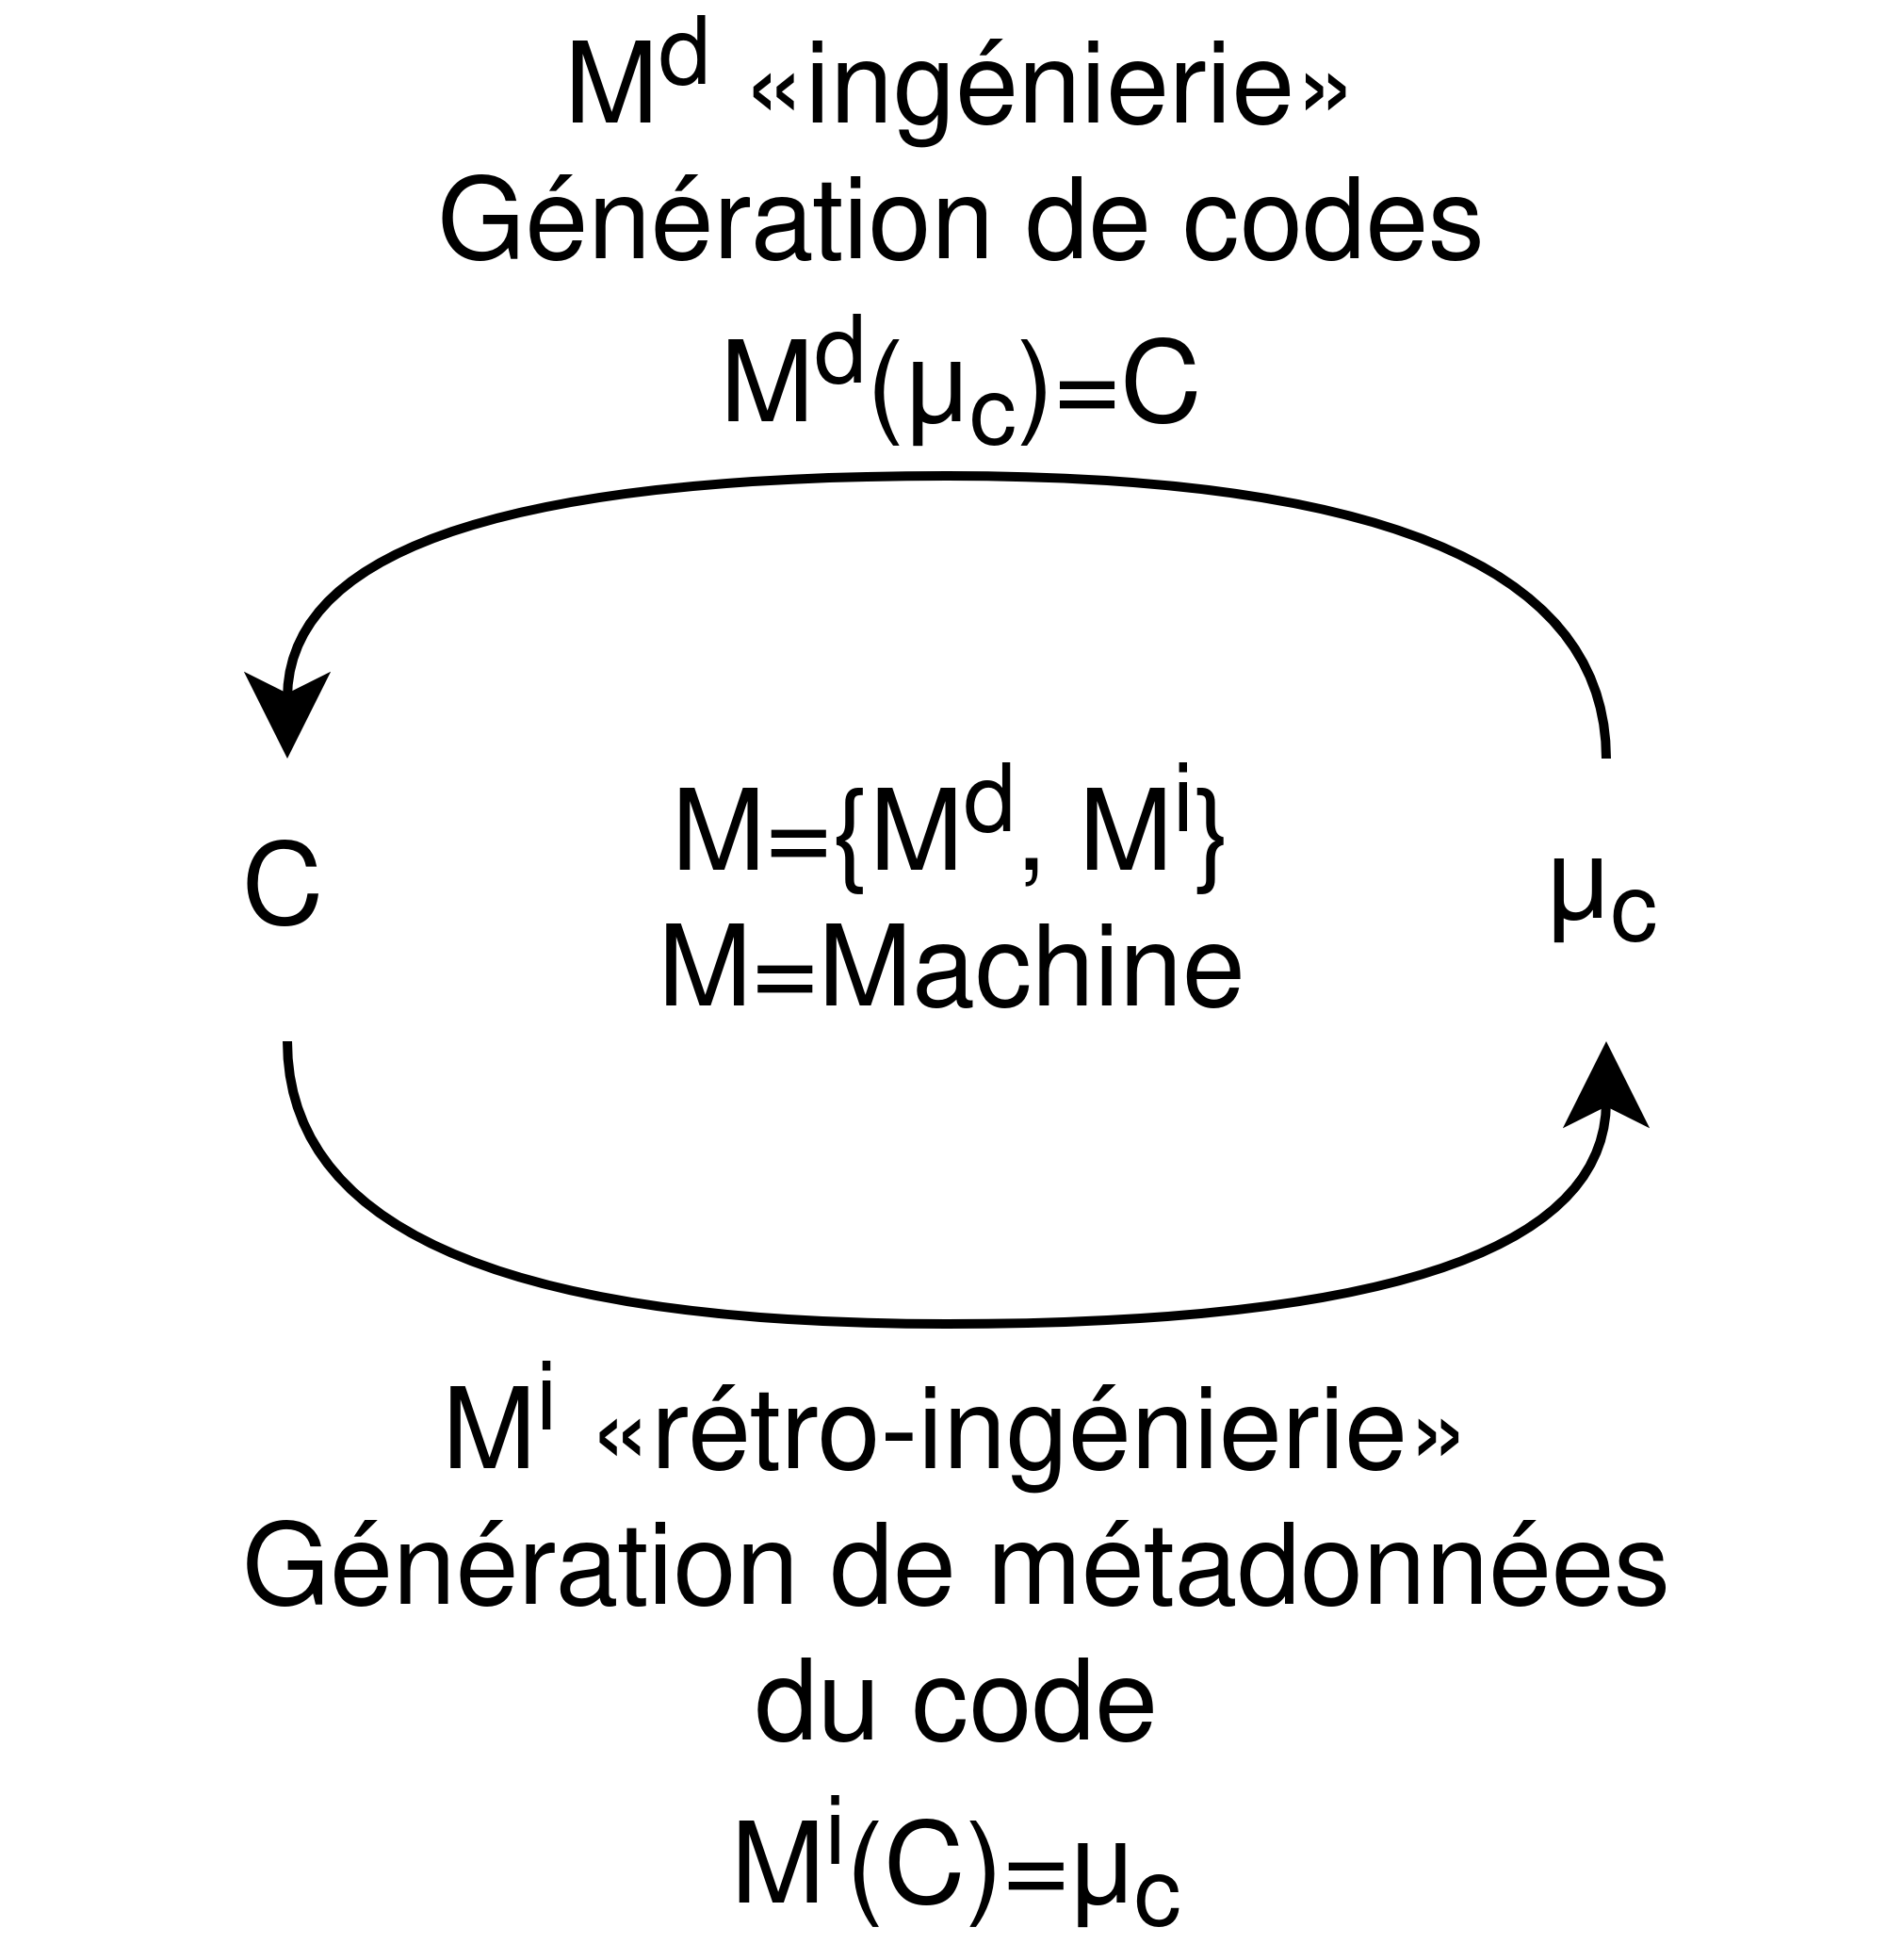
\includegraphics[width=2.5in]{images/machine_ing_retro_ing.drawio.png}
\caption{Mode direct et inverse}
\label{fig:mode_direct_inverse}
\end{figure}

Pour concrétiser le sens de ce modèle formel, nous allons proposer quelques exemples simples. Ayant pour but de faciliter la compréhension, ces exemples sont triviaux et ne présentent pas le plein potentiel de notre approche. L’interpréteur Python 3.6 et + est utilisé pour les exemples de codes.

Pour la plupart des exemples, le C, représenté par «C.py», est le code «Hello, World!», voir Figure~\ref{fig:exemple_code_hello_world}.

% \begin{lstlisting}[language=Python, upquote=false, caption={Exemple de code Hello, World!}, label={lst:exemple_code_hello_world}]
\begin{figure}
\begin{lstlisting}[language=Python]
print("Hello, World!")
\end{lstlisting}
\caption{Exemple de code Hello, World!}
\label{fig:exemple_code_hello_world}
\end{figure}

De plus, dans ce mémoire, nous utilisons le terme «générateur de code» qui est parfois représenté par «machine», cela fait référence à un ensemble de modules. Lorsque nous utilisons le terme robot logiciel codeur, nous faisons référence au «générateur de code» qui y est intégré, mais aussi à un ensemble de scripts dans ERPLibre, puisque le robot doit avoir un contrôle sur son projet en entier, jusqu'au déploiement de celui-ci. Ainsi, la machine est au niveau conceptuel théorique, le générateur de code est au niveau composante logicielle, et le robot logiciel codeur est au niveau de solution logicielle.

\subsection{Exemples illustratifs d’auto-reproducteur}\label{exemple_illustratif_auto_reproducteur}

\subsubsection{Le Quine}

«Un quine~\cite{sarkar2020quines} (ou programme auto-reproducteur, self-reproducing en anglais) est un programme informatique qui imprime son propre code source»~\cite{wiki_quine} sans se lire lui-même. Il doit contenir une logique d’écriture de code et contenir ses méta-données de génération. Il est ainsi un générateur de premier niveau.

Voir Figure~\ref{fig:exemple_quine}, la sortie textuelle dans la console, lors de l'exécution, est la même que son code.

\begin{figure}
\begin{lstlisting}[language=Python]
a='a=%r;print(a%%a)';print(a%a)
\end{lstlisting}
\caption{Exemple de code Quine}
\label{fig:exemple_quine}
\end{figure}

Cependant, le Quine ne sait rien faire d’autre que de s’auto-générer. Ce qui pourrait apporter une contribution serait de faire un auto-reproducteur qui permet de dériver vers d’autres fonctionnalités et ainsi intégrer l’amélioration continue sur son propre développement.

\subsection{Exemples illustratifs de générateur de code}

La génération de code est un des moyens pour soutenir le développeur dans le développement d’un logiciel. C’est la partie «création de code» de la méthodologie DevOps~\ref{devops_ref}.

\subsubsection{Technique de génération de code basique}

Dans Figure~\ref{fig:exemple_gen_code_basique}, la fonction «eval» en Python est dynamique, c'est-à-dire qu’elle permet l’exécution à partir d’une chaîne de caractères, ce type de génération de code ne permet pas une évolution efficace ou une simplification du développement. Ça revient à lire un fichier et à l'imprimer, il n’a pas de capacité dynamique d’adaptation.

\begin{figure}
\begin{lstlisting}[language=Python, upquote=true, caption={C de Figure~\ref{fig:exemple_gen_code_basique}}, label={lst:gen_code_basique_c}]
print("Hello, World!")
\end{lstlisting}

\begin{lstlisting}[language=Python, upquote=true, caption={µ$_C$ de Figure~\ref{fig:exemple_gen_code_basique}}, label={lst:gen_code_basique_uc}]
print('print("Hello, World!")')
\end{lstlisting}

\begin{lstlisting}[language=Python, upquote=true, caption={M(µ$_C$) de Figure~\ref{fig:exemple_gen_code_basique}}, label={lst:gen_code_basique_m}]
eval("""print('print("Hello, World!")')""")
\end{lstlisting}
\caption{Exemple de technique de génération de code basique d'un «Hello World»}
\label{fig:exemple_gen_code_basique}
\end{figure}

Dans Figure~\ref{fig:exemple_gen_code_basique_2}, cette technique basique est paramétrable, contrairement au premier exemple Figure~\ref{fig:exemple_gen_code_basique}. Le f-strings fait office de «template» et il y a la capacité dynamique d’adaptation en ajoutant des itérations et des conditions sans utiliser de bibliothèque externe.

\begin{figure}
\begin{lstlisting}[language=Python, upquote=true, caption={C - fichier C.py de Figure~\ref{fig:exemple_gen_code_basique_2}}, label={lst:gen_code_basique_2_c}]
print("Hello, World!")
\end{lstlisting}

\begin{lstlisting}[language=Python, upquote=true, caption={µ$_C$ - fichier uC.json de Figure~\ref{fig:exemple_gen_code_basique_2}}, label={lst:gen_code_basique_2_uc}]
{
 "fonction": "print",
 "argument": "\"Hello, World!\""
}
\end{lstlisting}

\begin{lstlisting}[language=Python, upquote=true, caption={M(µ$_C$) de Figure~\ref{fig:exemple_gen_code_basique_2}}, label={lst:gen_code_basique_2_m}]
import json

with open("uC.json") as f:
   metadata = json.load(f)

result = f"{metadata.get('fonction')}({metadata.get('argument')})\n"

with open("C.py", "w") as f:
   f.write(result)
\end{lstlisting}
\caption{Exemple de technique de génération de code basique paramétrable d'un «Hello World»}
\label{fig:exemple_gen_code_basique_2}
\end{figure}

\subsubsection{Technique de génération de code par «template»}

Un moteur de «template» est un outil de modèle structurel qui simplifie la syntaxe pour assurer une bonne maintenabilité et qui est généralement utilisé pour le développement de projet web.

La génération de code par «template» est une technique de développement de logiciels qui permet de produire du code source à partir de modèles prédéfinis appelés «template».

Le code de La Figure~\ref{fig:exemple_gen_code_basique_template} utilise la bibliothèque «Jinja2». C'est un mécanisme similaire à Figure~\ref{fig:exemple_gen_code_basique_2}, cependant la logique est intégrée directement dans le fichier template.

\begin{figure}
\begin{lstlisting}[language=Python, upquote=true, caption={C - fichier C.py de Figure~\ref{fig:exemple_gen_code_basique_template}}, label={lst:gen_code_template_c}]
print("Hello, World!")
\end{lstlisting}

\begin{lstlisting}[language=Python, upquote=true, caption={µ$_C$ - fichier uC.json de Figure~\ref{fig:exemple_gen_code_basique_template}}, label={lst:gen_code_template_uc}]
{
 "fonction": "print",
 "argument": "\"Hello, World!\""
}
\end{lstlisting}

\begin{lstlisting}[language=Python, upquote=true, caption={template - fichier template de Figure~\ref{fig:exemple_gen_code_basique_template}}, label={lst:gen_code_template_template}]
{{ fonction }}({{ argument }})
\end{lstlisting}

\begin{lstlisting}[language=Python, upquote=true, caption={M(µ$_C$) de Figure~\ref{fig:exemple_gen_code_basique_template}}, label={lst:gen_code_template_m}]
import json

from jinja2 import Template

with open("template") as f:
   template = Template(f.read())

with open("uC.json") as f:
   metadata = json.load(f)

result = template.render(
   fonction=metadata.get("fonction"), argument=metadata.get("argument")
)

with open("C.py", "w") as f:
   f.write(result)
\end{lstlisting}
\caption{Exemple de technique de génération de code par template avec Jinja2 d'un «Hello World»}
\label{fig:exemple_gen_code_basique_template}
\end{figure}

% Les avantages du template~\ref{fig:gen_code_template_template_2} pour cette approche sont : une productivité accrue, une réduction des erreurs de codage, une meilleure cohérence du code et une réduction du temps de développement. Cette technique peut également faciliter la maintenance du code, puisque les modifications apportées aux templates sont automatiquement propagées à tout le code généré.

\begin{figure}
\begin{lstlisting}[language=Python]

  <li>
	:):(
	<em>{{ student.name }}:</em> {{ student.score }}/{{ max_score }}
  </li>

\end{lstlisting}
\caption{Exemple de template Jinja2 avec logique}
\label{fig:gen_code_template_template_2}
\end{figure}


\subsubsection{Générateur de code par template avec Odoo 12}

La technique utilisée par Odoo 12 est le «scaffold», il gère 2 types de «template» : un module de base «default» et un module thème «theme».

Dans Figure~\ref{fig:exemple_odoo_scaffold_module}, tout est presque commenté, rien n’est utilisable, mais nous avons la structure MVC. Le gain d’accélération au développement est minime.

\begin{figure}
\begin{lstlisting}[language=Python]
> ./odoo/odoo-bin scaffold module_default ./
> tree module_default/
controllers
    controllers.py
    __init__.py
demo
    demo.xml
__init__.py
__manifest__.py
models
    __init__.py
    models.py
security
    ir.model.access.csv
views
    templates.xml
	views.xml
\end{lstlisting}
\caption{Exemple de génération de module MVC Odoo avec la technique du Scaffold}
\label{fig:exemple_odoo_scaffold_module}
\end{figure}

Cette fois-ci, dans Figure~\ref{fig:exemple_odoo_scaffold_theme}, tout est vide, le module «theme\_module» produit une erreur à l'installation. Il est plus efficace de copier et de modifier un thème existant que d'utiliser le «scaffold».

\begin{figure}
\begin{lstlisting}[language=Python]
> /odoo/odoo-bin scaffold -t theme theme_module ./
> tree theme_module/
demo
    pages.xml
__init__.py
__manifest__.py
static
    src
        scss
            custom.scss
views
    options.xml
    snippets.xml
\end{lstlisting}
\caption{Exemple de génération de module thème Odoo avec la technique du Scaffold}
\label{fig:exemple_odoo_scaffold_theme}
\end{figure}

Le gain d’accélération au développement peut être considéré comme négligeable. Copier un module fonctionnel et l'adapter est plus efficace. Admettons que cette technique est utile pour un débutant, pour comprendre à quoi ressemble une architecture vide, mais il va apprendre plus vite en regardant le fonctionnement de module fonctionnel ou lire la documentation officielle sur comment développer un module Odoo.

\subsubsection{Technique de génération de code par rétro-ingénierie}

Lorsqu'on veut faire de la rétro-ingénierie~\cite{wikipedia_retroingenierie} avec un générateur de code, l'objectif est de faire de la ré-ingénierie sur la partie génération, ainsi on altère le code, voir Figure~\ref{fig:retro_re_ing}.

\begin{figure}[htb]
\centering
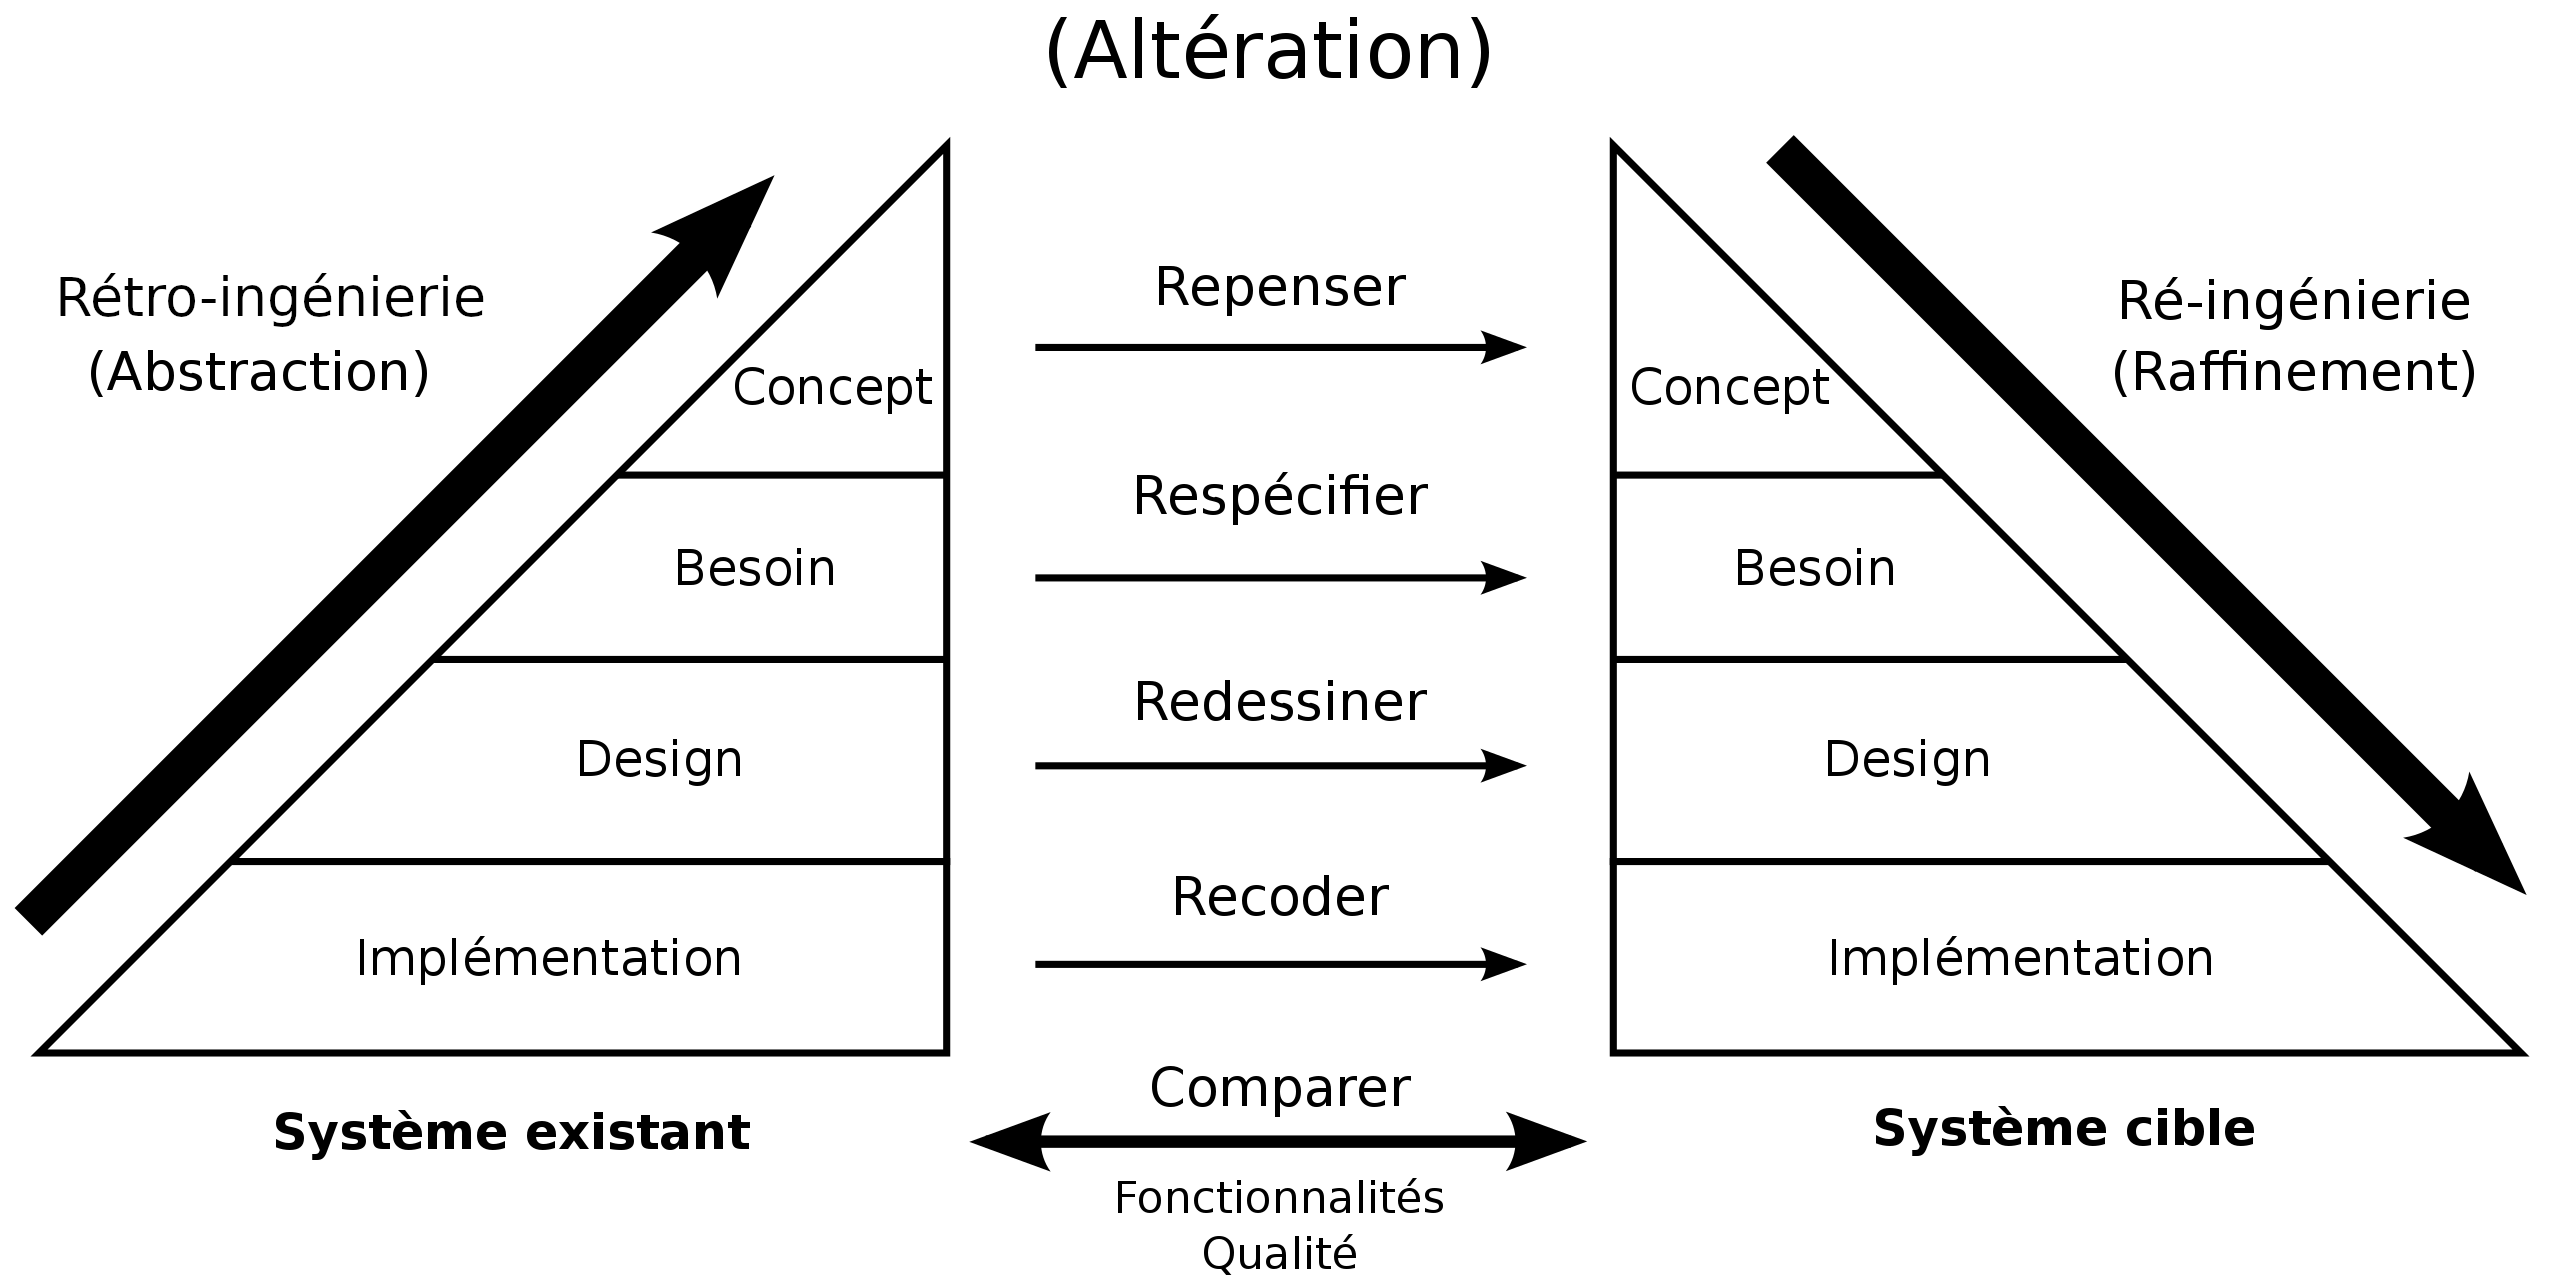
\includegraphics[width=5in]{images/Retroingenierie_-_Byrne.png}
\caption{Altération du code avec la rétro-ingénierie et la ré-ingénierie. Image modifiée~\cite{wikipedia_image_retroingenierie}}
\label{fig:retro_re_ing}
\end{figure}

Dans Figure~\ref{fig:exemple_gen_code_retro}, le code~\ref{lst:gen_code_retro_m} utilise la bibliothèque AST pour analyser l’arbre de syntaxe abstraite du code source. La difficulté avec la rétro-ingénierie est de savoir précisément ce qu’on cherche à extraire; il faut avoir un cas d’utilisation spécifique. Ici, le cas d’utilisation est la recherche d’un nœud de type expression qui contient des paramètres. L’avantage est de permettre de corriger des problèmes de qualité logicielle entre l’extraction d’information et la génération du code. Dans ce contexte, le résultat~\ref{lst:gen_code_retro_new_c} du code source original~\ref{lst:gen_code_retro_c} devient formaté en PEP8~\cite{python_pep8}.

\begin{figure}
\begin{lstlisting}[language=Python, upquote=true, caption={C mal formaté - fichier C.py de Figure~\ref{fig:exemple_gen_code_retro}}, label={lst:gen_code_retro_c}]
print(                     "Hello, World!"                         )
\end{lstlisting}

\begin{lstlisting}[language=Python, upquote=true, caption={M qui extrait µ$_C$ pour générer C.py de Figure~\ref{fig:exemple_gen_code_retro}}, label={lst:gen_code_retro_m}]
import ast

with open("C.py", "r") as f:
   code = f.read()

# Extraction du AST
tree = ast.parse(code)
node = tree.body[0]

if (
   isinstance(node, ast.Expr)
   and isinstance(node.value, ast.Call)
   and isinstance(node.value.func, ast.Name)
):
   # Si une expression executable de type function est trouve
   fct_arg = ""
   for arg in node.value.args:
       if isinstance(arg, ast.Str):
           # Cherche un parametre
           fct_arg = arg.s
           break
   # Template
   result = f"""{node.value.func.id}("{fct_arg}")\n"""

with open("C.py", "w") as f:
   f.write(result)
\end{lstlisting}

\begin{lstlisting}[language=Python, upquote=true, caption={C corrigé - fichier C.py de Figure~\ref{fig:exemple_gen_code_retro}}, label={lst:gen_code_retro_new_c}]
print("Hello, World!")
\end{lstlisting}
\caption{Exemple de technique de génération de code avec rétro-ingénierie d'un «Hello World»}
\label{fig:exemple_gen_code_retro}
\end{figure}

\subsection{Tester un générateur de code}

Il existe le test «Output comparison testing»~\cite{wikipedia_test_informatique} qui est le principe que le générateur de code crée du code (une sortie en texte lisible par l'humain) et que l'humain valide cette sortie textuelle.

Pour valider si le générateur utilise sa pleine capacité, il suffit de faire des tests de toutes les combinaisons de ses techniques de génération et d'utiliser un outil de couverture de code pour déterminer les lignes qui sont opérées.

% TODO missing auto-ingénierie, auto-amélioration, évolution technique rétro


% Exemple
% Texte en \emph{italique}, \textsc{petites majuscules}, mot \mbox{insécable}.\\
% Texte \ul{souligné}, \hl{surligné}, \textbf{gras}.\\
% Texte entre ``guillemets''.\\
% Police \texttt{monospace}.\\
% Un mot courant en réseautique mobile: n\oe{}ud\footnote{Note de bas de page.}.\\
% L'objet RSVP \texttt{SENDER\_TEMPLATE}.\\
% Nom d'un auteur: \citeauthor{RFC_IPv4}.\\
% Une architecture 32~bits.\\
%%
%%  CONCEPTS DE BASE / BASIC CONCEPTS
%%
% \section{Définitions et concepts de base}  % environ 2-3 pages
% \begin{flushleft}
% 1\iere{} utilisation d'un acronyme yeah: \ac{IETF}.\\
% 2\ieme{} utilisation d'un acronyme: \ac{IETF}.\\ ça ne marche pas
% Acronyme au long: \acl{IETF}.\\
% \end{flushleft}

% \subsection{Une sous-section}
% Un URL: \href{http://www.polymtl.ca}{École Polytechnique de Montréal}.

% \subsubsection{Une sous-sous-section}
% Les besoins des flots de données peuvent être catégorisés selon
% quatre paramètres importants \cite{Fraas2010} ou:
% \begin{itemize}
% \item la fiabilité (acheminement des données avec succès)~;
% \item le délai de \mbox{bout-en-bout} de la source vers la destination~;
% \item la variation du délai de \mbox{bout-en-bout} (\emph{jitter})~;
% \item la bande passante requise (le débit des informations).
% \end{itemize}

% \paragraph{Le niveau paragraphe} est plus bas encore dans la hiérarchie\ldots
% Une citation entre parenthèses \cite{SAHIN2020}.
% ou des citations entre parenthèses \cite{Haist2014,Senjian2015,Madani2010}.

% \clearpage

% %%
% %% ELEMENTS DE LA PROBLEMATIQUE
% %%
% \section{Éléments de la problématique}  % environ 3 pages
% La description de \mbox{l'en-tête} commun de RSVP est détaillée ci-dessous:\\
% \begin{tabular}{p{1in}p{4.5in}}
% &\\ % Ligne vide
% \texttt{Ver}: & \texttt{4 bits}\\
%           & Version du protocole. La version actuelle est~1.\\[5pt]
% \texttt{Flags}: & \texttt{4 bits}\\
%           & Aucun Flag n'est défini. L'émetteur doit (\textbf{MUST})
%           mettre le champ à zéro et le récepteur doit (\textbf{MUST})
%           ignorer ce champ.\\[5pt]
% \texttt{Msg Type}: & \texttt{8 bits}\\
%           & Type de message\\[5pt]
% \texttt{Checksum}: & \texttt{16 bits}\\
%           & Complément à un du complément à un de la somme des champs
%           de \mbox{l'en-tête}, avec le champ Checksum à~0 pour des
%           fins de calcul. La valeur~0 signifie qu'aucun Checksum n'a
%           été transmis. Si le résultat du calcul du Checksum donne~0,
%           la valeur 0xFFFF doit être stockée dans ce champ.\\[5pt]
% \texttt{TTL}: & \texttt{8 bits}\\
%           & Valeur originelle du champ \texttt{TTL} utilisée pour
%           transmettre ce message.\\[5pt]
% \texttt{Reserved}: & \texttt{8 bits}\\
%           & Réservé pour usage futur. L'émetteur doit (\textbf{MUST})
%           mettre le champ à zéro et le récepteur doit (\textbf{MUST})
%           ignorer ce champ.\\[5pt]
% \texttt{Length}: & \texttt{16 bits}\\
%           & Longueur totale du message en octets, incluant
%           \mbox{l'en-tête} commun et tous les objets de longueur
%           variable.
% \end{tabular}

% \subsection{Autres types de structures de données}
% L'énumération:
% \begin{enumerate}
% \item Un item~;
% \item Un autre item.
% \end{enumerate}


% \subsection{Le protocole IPv6}
% Voir la Figure~\ref{fig:IPv6} pour plus de détails. Le champs DSCP est
% décrit dans le Tableau~\ref{tab:RangesDSCP}.

% \begin{figure}[htb]
% % [htb] place la figure ici + en haut ou en bas de la page. 
% % [htb] places the figure here + top or bottom of the page. 
% % Vous pouvez également utiliser [tb] pour placer les figures en haut ou en bas de la page et [p] pour les placer sur une page ne contenant que des flottants (ex. : tableaux, figures).
% % You can also use [tb] for placing figures on the top or the bottom of a page and [p] for a figure placed on a page containing only floats (ex.: tables, figures).
% % Plus d'informations / More information here: https://www.ctan.org/tex-archive/info/epslatex/english 
% \centering
% 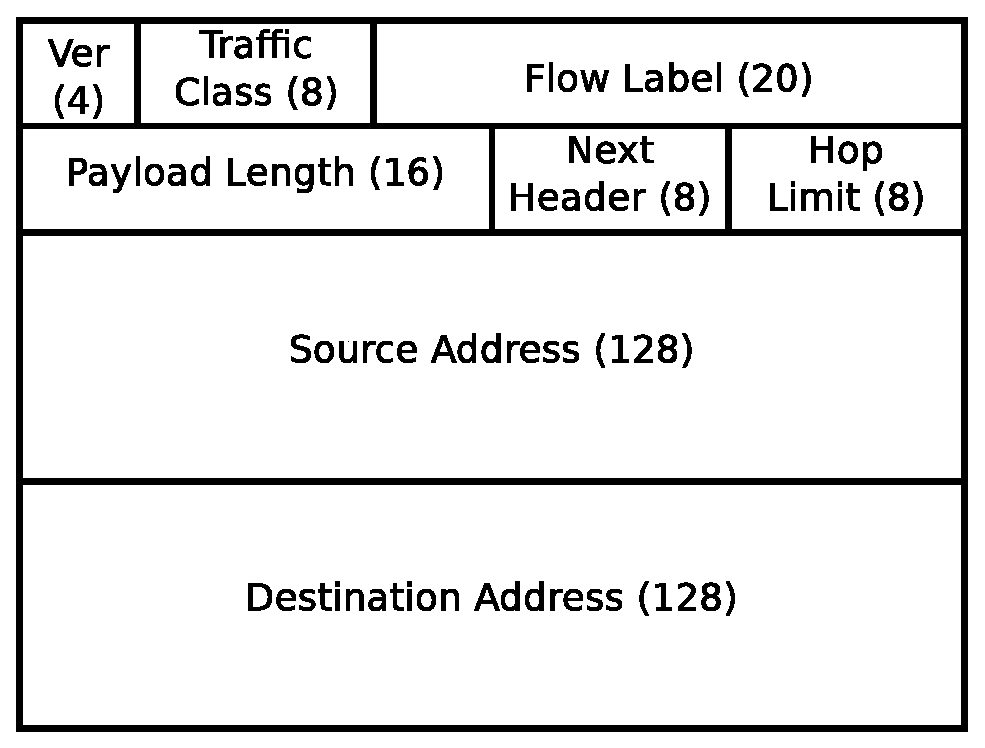
\includegraphics[width=4in]{IPv6_header}
% \caption{L'en-tête IPv6}
% \label{fig:IPv6}
% \end{figure}

% \begin{table}[htb]
% \caption{Plages de valeurs pour le champ \texttt{DSCP}}
% \centering
% \begin{tabular}{|c|c|l|}
% \hline\rowcolor[gray]{0.8}\color{black}
% Plage & Valeurs & Règle d'assignation\\\hline
% 1 & xxxxx0 & Assignation par une norme de l'IANA\\\hline
% 2 & xxxx11 & Expérimentation/Usage local\\\hline
% 3 & xxxx01 & Expérimentation/Usage local (pourrait être jointe à la plage 1)\\\hline
% \end{tabular}
% \label{tab:RangesDSCP}
% \end{table}

% % On veut éviter que la figure et le tableau soient placés au-delà de la section courante.
% % To prevent the figure and table from being positioned outside of the current section. 
% \FloatBarrier


% %%
% %% OBJECTIFS DE RECHERCHE / RESEARCH OBJECTIVES
% %%
% \section{Objectifs de recherche}  % 0.5 page
% Les objectifs de la recherche sont de concevoir un algorithme $O(n)$.


% %%
% %% PLAN DU MEMOIRE / THESIS OUTLINE
% %%
% \section{Plan du mémoire}  % 0.5 page

% Voir la Figure~\ref{fig:Layers} pour plus de détails. 

% \begin{figure}[htb]
% \centering
% 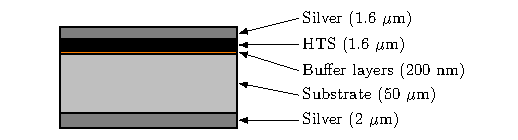
\includegraphics[width=4in]{demo_tikz}
% \caption{Couches}
% \label{fig:Layers}
% \end{figure}


% Un tableau : / A table:
% \begin{table}[htb]
%   \centering
%   \caption{Constantes et variables du modèle analytique}
%   \begin{tabular}{|c|l|}
%     \hline\rowcolor[gray]{0.8}\color{black}
%     Symbole         & Description\\\hline
%     $\lambda$       & Taux d'arrivée moyen des requêtes de réservation de ressources\\\hline
%     $\frac{1}{\mu}$ & Durée moyenne d'une session\\\hline
%     $C$             & Capacité d'une cellule (nombre de sessions supportées)\\\hline
%     $v_{moy}$       & Vitesse moyenne des MN dans le réseau d'accès\\\hline
%     $L$             & Longueur d'un côté d'une cellule carrée\\\hline
%     $n$             & Nombre moyen de MN dans une cellule\\\hline
%     $\rho$          & Charge d'une cellule\\\hline
%     $P_b$           & Probabilité de blocage d'une requête de réservation\\\hline
%     $P_f$           & Probabilité d'interruption forcée d'une session\\\hline
%     $P_c$           & Probabilité de compléter une session avec succès\\\hline
%     $\Delta{}T$     & Délai de transmission\\\hline
%   \end{tabular}
%   \label{tab:Definitions}
% \end{table}

% La formule d'\mbox{Erlang-B}:
% \begin{equation}
%   P_b = \frac{\frac{\rho^C}{C!}}{\sum\limits_{x=0}^{C}\frac{\rho^x}{x!}}
%   \label{eq:Pblock}
% \end{equation}

% Une autre équation : / Another equation:
% \begin{equation}
%   \begin{split}
%     P_c &= (1 - P_b) \times (1 -  P_f)^N\\
%         &= (1 - P_b)^{N+1}
%   \end{split}
%   \label{eq:ProbComplete}
% \end{equation}

% Enfin, l'expression suivante indique le moment à partir duquel les
% réservations de ressources sont en place:
% \begin{equation}
%   \Delta{}T_{init} =
%   \begin{cases}
%     2\Delta{}T_{E2E} & \Delta{}T_{wan} > (\Delta{}T_{rad} + \Delta{}T_{net})\\
%     \Delta{}T_{E2E} + 3(\Delta{}T_{rad} + \Delta{}T_{net}) & \text{sinon}
%   \end{cases}
%   \label{eq:InitCost}
% \end{equation}

% \paragraph{Le taux de paquets perdus} correspond au nombre de paquets
% éliminés à cause d'une erreur de \emph{checksum} à un n\oe{}ud
% quelconque ou d'une situation de congestion. Le taux de paquets perdus
% pour un chemin est déterminé de la façon suivante:
% \begin{equation}
%   \label{eq:genPLR}
%   PLR_P = 1 - \prod_{i=1}^N(1 - PLR_i)
% \end{equation}

% Toutefois, si les taux d'erreurs sont très faibles, comme c'est
% généralement le cas pour des liens optiques, on peut approximer
% $PLR_P$ de façon à le transformer en un paramètre additif:
% \begin{equation}
%   \label{eq:approxPLR}
%   \begin{split}
%     PLR_{L_1 \oplus L_2} &= 1 - (1 - PLR_1)(1 - PLR_2)\\
%     &= 1 - (1 - PLR_2 - PLR_1 + \underbrace{PLR_1
%       \times PLR_2}_\text{négligeable})\qquad PLR_1 \ll 1,
%     PLR_2 \ll 1\\
%     &\approx PLR_1 + PLR_2
%   \end{split}
% \end{equation}

% \clearpage

% Une courbe : / A curve:
% \begin{figure}[htb]
% \centering
% 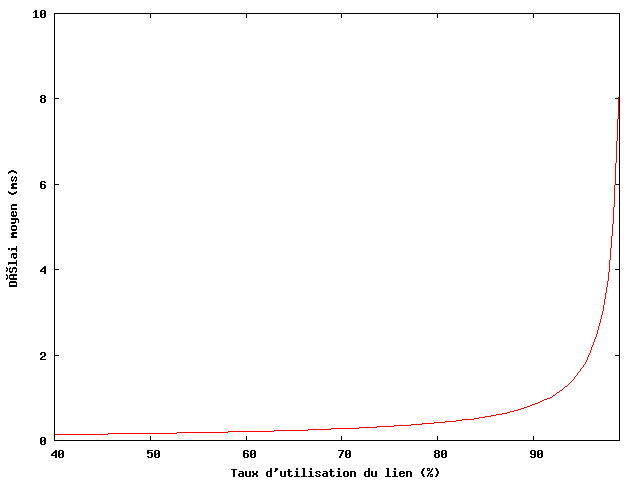
\includegraphics[width=5in]{LinkUsage}
% \caption{Délai moyen en fonction du taux d'utilisation d'un lien}
% \label{fig:LinkUse}
% \end{figure}

% \selectlanguage{english}
% This paragraph is formatted by \LaTeX{} according to the standard rules of the
% English language (\mbox{e.g.} hyphenation).
% \selectlanguage{french}

% L'arithmétique en virgule flottante peut entraîner des erreurs
% d'approximation et il est important d'en être conscient
% \cite{Rossi2011}.

% De même, les calculs effectués sur une carte graphique (GPU) peuvent
% introduire des erreurs d'approximation \cite{DeSantis2002, Cohen2006,
%   Thorsson2014, Schirmer2012, Sakai2015, Electrical2006,
%   Min2016, Massicotte2013, Kaliouby1987, Daintith2010, Haist2014, Kizza2013,
%   Manasreh2011, Brydson1999, Boyce2002}.
